\documentclass[11pt,a4paper]{article}
\usepackage[margin=2.5cm]{geometry}
\usepackage{graphicx}
\usepackage{booktabs}
\usepackage{amsmath}
\usepackage{caption}
\usepackage{xcolor}
\usepackage{float}
\usepackage[colorlinks=true,linkcolor=blue!50!black,citecolor=blue!50!black,urlcolor=blue!50!black]{hyperref}
\graphicspath{{../figures/}}
\setlength{\parskip}{0.5em}
\setlength{\parindent}{0pt}

\title{Machine-Learning Fault Detection, Classification and Location\\on a Simulated 220\,kV Transmission Line}
\author{Ludwig S Ben-Acquaah}
\date{October 2026}

\begin{document}
\maketitle

\begin{abstract}
Transmission-line faults must be detected quickly, and knowing the fault type and approximate distance helps crews restore supply faster. This project builds a MATLAB/Simulink model of a 220\,kV, 60\,Hz, 40\,km line, runs 2000 randomised simulations (faults and no-fault cases), and trains machine-learning models to detect, classify and locate faults from sending-end voltage and current alone. A current-RMS trigger detects every fault within 6.6\,ms. A Random Forest classifies fault type with 99.4\% accuracy on an independent test set whose conditions (load, power factor, fault resistance, location range, noise) were not in the training data, and an Extra Trees regressor locates faults with a mean error of 1.82\,km (median 0.71\,km, 4.6\% of the line). Accuracy degrades for fault resistance above the training range, which we measure and discuss. All results come from simulation of one line model, and the limitations are stated explicitly.
\end{abstract}

\section{Introduction}
Electricity travels long distances through transmission lines, and a fault can interrupt supply and damage equipment. A monitoring system should therefore do more than report that ``something is wrong'': it should say what kind of fault occurred and roughly where. This project asks how well simple, interpretable machine-learning models can do that from measurements at one end of a line.

The contributions are: (i) a validated Simulink model with a randomised fault-injection pipeline; (ii) a trigger and feature-extraction chain that does not depend on knowing the true fault time; (iii) a Random Forest fault-type classifier and an Extra Trees fault locator; and (iv) an evaluation that includes an independent out-of-distribution test set, stress tests, an ablation study and a classical baseline, with explicit limitations.

An earlier version of the dataset gave 100\% accuracy. Inspection showed that the simulated no-fault signals were numerically perfect, that analysis windows were aligned to the true fault time, and that there was no independent test. The work reported here is the corrected second version (Section~\ref{sec:v2}).

\section{Background}
\subsection{Short-line model}
For a short line (shunt capacitance neglected) the sending-end phasor voltage is $V_S = V_R + I_R Z$, with $Z = R + jX_L$. With the receiving-end voltage at 220\,kV line-to-line and a 381\,MVA, 0.8 power factor lagging load, $I_R \approx 1000$\,A and the line impedance is $Z = 6 + j20\ \Omega$ (40\,km at $0.15\ \Omega$/km and $0.5\ \Omega$/km at 60\,Hz). This gives $|V_{S,\phi}| \approx 144.4$\,kV (250.1\,kV line-to-line), voltage regulation of about 13.7\% and efficiency of 94.4\%. The Simulink model reproduced these values (13.6\% regulation, 94.42\% efficiency). An initial hand calculation had given 243.1\,kV and 10.5\%; this was an arithmetic error that the simulation exposed, and the corrected values above agree with the simulation.

\subsection{Fault types and symmetrical components}
Four short-circuit types are considered: single line-to-ground (LG), line-to-line (LL), double line-to-ground (LLG) and three-phase (LLL). Fortescue's method~\cite{fortescue1918} decomposes three phasors into zero-, positive- and negative-sequence components,
\begin{equation}
 I_0 = \tfrac{1}{3}(I_a+I_b+I_c),\quad I_1 = \tfrac{1}{3}(I_a+aI_b+a^2I_c),\quad I_2 = \tfrac{1}{3}(I_a+a^2I_b+aI_c),
\end{equation}
with $a = e^{j2\pi/3}$. A balanced system has only $I_1$. Faults involving ground produce $I_0$, unbalanced faults produce $I_2$, and the pattern identifies the type (Figure~\ref{fig:sep}).

\subsection{Fault location from apparent impedance}\label{sec:locbg}
At the sending end, the impedance seen to a fault at distance $d$ is approximately $d\,z_L + R_f$, where $z_L$ is the line impedance per kilometre and $R_f$ the fault resistance. Reactance, $d \cdot 0.5\ \Omega$/km here, is largely independent of $R_f$, whereas the magnitude of the impedance is not. A model that sees only magnitudes confuses distance with fault resistance. This motivates the resistance and reactance features in Section~\ref{sec:features}~\cite{saha2010}.

\section{Simulation}
\subsection{Model}
Figure~\ref{fig:system} shows the system. A three-phase source (263.1\,kV line-to-line, $1 + j10\ \Omega$ internal impedance, so that the sending-end voltage stays near 144.3\,kV per phase) feeds a 40\,km lumped RL line split into two sections, \texttt{Line1} (length $d$) and \texttt{Line2} (length $40-d$), with a three-phase fault block at the join. The load is 381\,MVA at 0.8 power factor lagging. The model was built with Simscape Electrical in Simulink, run in discrete mode at 360 samples per cycle (21.6\,kHz) for 0.25\,s.

\begin{figure}[H]\centering
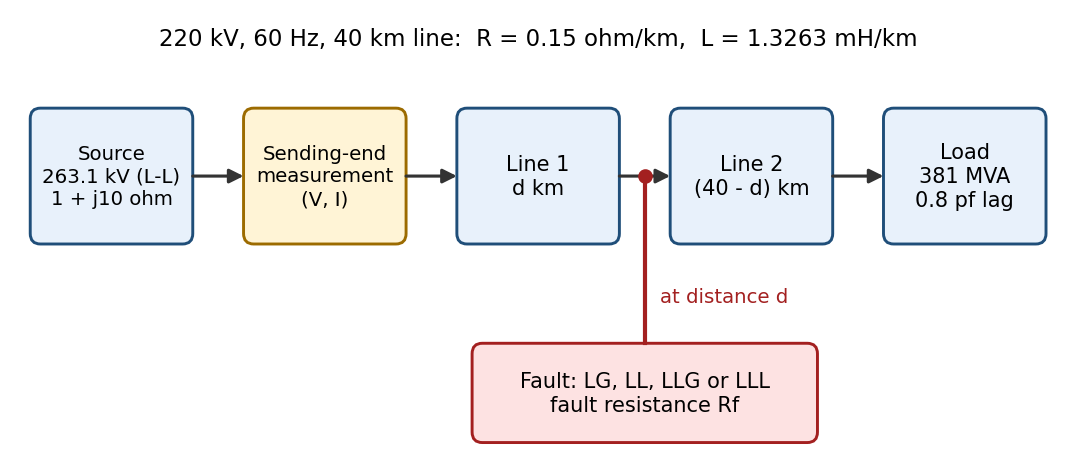
\includegraphics[width=\textwidth]{fig_system.png}
\caption{Simulated system. The fault block sits at a random distance $d$ from the sending end; voltages and currents are measured at the sending end only.}\label{fig:system}
\end{figure}

\subsection{Randomised fault generation}
Each run draws a fault class, the phases involved, fault distance, fault resistance, inception time and load level. Ground resistance is fixed at 0.01\,$\Omega$, so $R_f$ is the resistance in each faulted phase. Table~\ref{tab:sets} lists the ranges. No-fault runs use the same load variation. The independent set uses a different random seed and wider conditions.

\begin{table}[H]\centering\small
\caption{Training and independent datasets.}\label{tab:sets}
\begin{tabular}{lll}\toprule
 & Training & Independent test\\\midrule
Runs & 1500 (300 per class) & 500 (100 per class)\\
Random seed & 42 & 7\\
Fault distance & 2--38\,km & 1--39\,km\\
Fault resistance & 0.01--50\,$\Omega$ (log-uniform) & 0.01--100\,$\Omega$ (log-uniform)\\
Load & P and Q scaled together, 0.8--1.2 & P 0.5--1.3, Q 0.5--1.5, independent\\
Measurement errors and noise & 1$\times$ & 1.5$\times$\\\bottomrule
\end{tabular}
\end{table}

\subsection{Measurement imperfections}
To avoid numerically perfect signals, each run applies a fixed gain error to every channel (voltage $\pm0.5\%$, current $\pm1\%$, uniform) and adds Gaussian noise with standard deviation 0.2\% of the nominal peak value (204\,kV and 1414\,A). The independent set scales all of these by 1.5. CT saturation and harmonics are not modelled.

\section{Detection and feature extraction}\label{sec:features}
\subsection{Trigger and windows}
A fault is detected when the one-cycle RMS of any phase current reaches 1.3 times its value one cycle earlier; the search starts at 0.1\,s to skip start-up transients. The trigger does not use the true fault time. The \emph{pre-fault window} is the cycle ending one cycle before the trigger, and the \emph{post-fault window} is the cycle starting at the trigger. Phasors are obtained with a one-cycle discrete Fourier transform. For no-fault runs an arbitrary pseudo-event time is used when the trigger does not fire.

\subsection{Features}
There are 37 features per run (Table~\ref{tab:feat}); the locator adds 10 derived impedance features. Fault type, phases, resistance, distance and inception time are never given to the models as inputs.

\begin{table}[H]\centering\small
\caption{Feature groups.}\label{tab:feat}
\begin{tabular}{ll}\toprule
Group & Description\\\midrule
Magnitudes (6) & Post-fault phase voltage and current magnitudes\\
Ratios (6) & Post-fault over pre-fault magnitude, per phase\\
Sequence (6) & Zero-, positive-, negative-sequence voltage and current\\
Sequence ratios (5) & $I_0/I_1$, $I_2/I_1$, $V_1/I_1$, $V_2/I_2$, $V_0/I_0$\\
Phase impedance (6) & Resistance and reactance of $V_\phi/I_\phi$\\
Loop impedance (6) & Resistance and reactance of $V_{ab}/(I_a-I_b)$, etc.\\
Positive-sequence impedance (2) & Resistance and reactance of $V_1/I_1$\\\bottomrule
\end{tabular}
\end{table}

\begin{figure}[H]\centering
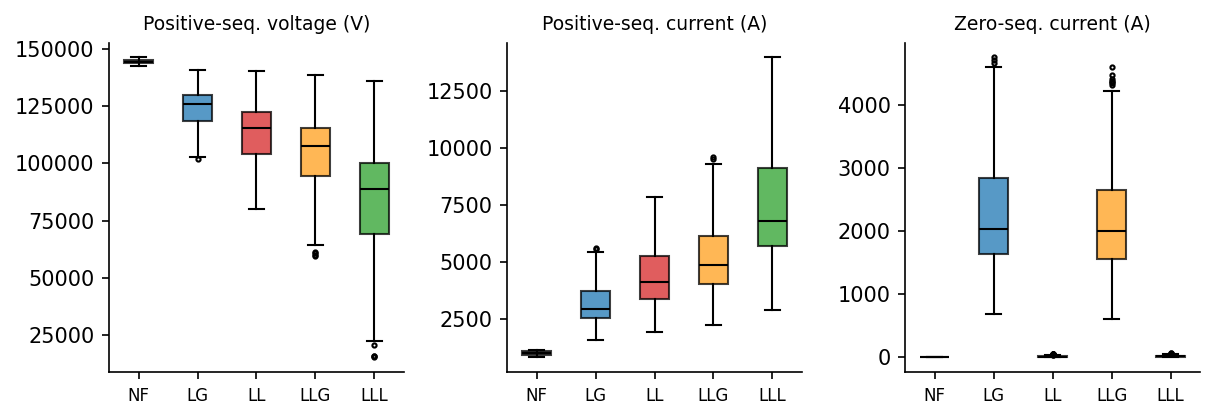
\includegraphics[width=\textwidth]{fig_separability.png}
\caption{Distribution of three features by class (training set). Ground faults produce a large $I_0$; no-fault runs sit near zero.}\label{fig:sep}
\end{figure}

\section{Models and evaluation protocol}
\textbf{Classifier.} A Random Forest~\cite{breiman2001} with 300 trees assigns one of five classes (NF, LG, LL, LLG, LLL). \textbf{Locator.} An Extra Trees regressor~\cite{geurts2006} with 400 trees estimates $d$ from fault runs only. Both use scikit-learn~\cite{pedregosa2011}.

The evaluation has four parts. (1) A same-distribution test: 20\% of the training set held out (300 runs), plus five-fold cross-validation and five random splits for location. (2) The \emph{independent test set} of 500 runs, with models trained only on the training set. (3) Stress tests on the training set: training only on $R_f \le 10\ \Omega$ and testing above, and holding out the 3--10\,$\Omega$ band. (4) An ablation study of the resistance and reactance features and a classical baseline. Where zero errors occur in $n$ trials, the 95\% upper bound on the error rate is approximately $3/n$.

\begin{figure}[H]\centering
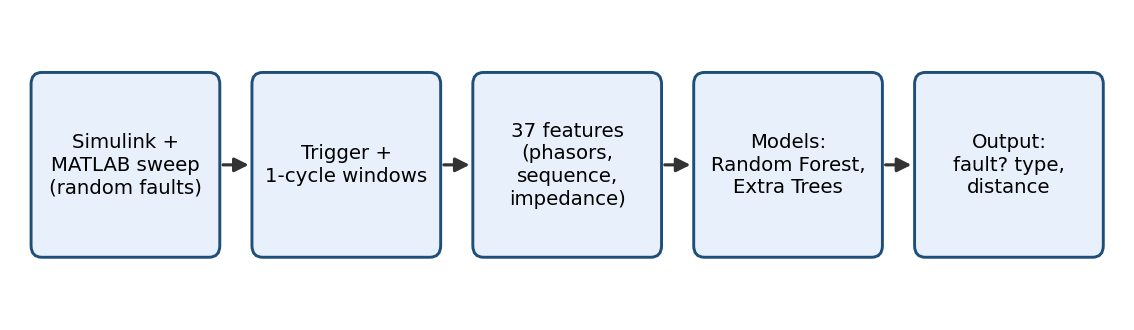
\includegraphics[width=0.9\textwidth]{fig_pipeline.png}
\caption{Processing pipeline.}\label{fig:pipe}
\end{figure}

\section{Results}
\subsection{Simulation versus circuit theory}
For low-resistance faults ($R_f<5\ \Omega$) the peak phase current at the sending end was compared with the steady-state formula $E/|Z_s + d z_L + R_f|$ (and $\sqrt3E/2|Z_s+dz_L+R_f|$ for LL), using $Z_0 = Z_1$ as in the model (Table~\ref{tab:theory}). The simulated value is about 8--12\% higher, which is the size expected from the decaying DC offset in the first cycle after the fault (a simple RL-transient calculation gives 1.1--1.2 times the steady-state RMS). This is consistent with the theory but is not an exact transient comparison.

\begin{table}[H]\centering\small
\caption{Simulated divided by analytic fault current.}\label{tab:theory}
\begin{tabular}{lrcc}\toprule
Type & Runs & Median ratio & 10th--90th percentile\\\midrule
LLL & 228 & 1.11 & 1.09--1.13\\
LG & 214 & 1.08 & 0.95--1.14\\
LL & 219 & 1.12 & 0.99--1.18\\\bottomrule
\end{tabular}
\end{table}

\subsection{Detection}
The trigger missed 0 of 1200 training faults and raised 0 false alarms in 300 no-fault runs. On the independent set it missed 0 of 400 faults with 0 false alarms in 100 no-fault runs. The median detection delay was 1.4\,ms and the maximum 6.6\,ms, well under one 16.7\,ms cycle. This applies to faults against steady-state operation; non-fault disturbances were not simulated.

\subsection{Fault-type classification}
On the same-distribution test the Random Forest classified all 300 held-out runs correctly (five-fold cross-validation 100.0\% $\pm$ 0.0\%). A depth-4 decision tree on three features also reaches 100.0\%, so type classification is easy on this simulator: the sequence components separate the classes with large margins (ground-fault $I_0$ is at least about 600\,A, line-to-line $I_0$ at most about 60\,A, and no-fault values are a few amperes).

On the independent test the accuracy was 99.4\% (497 of 500, 95\% confidence interval 98.3--99.9\%). The three errors all had fault resistance of 85--94\,$\Omega$, beyond the 50\,$\Omega$ training limit (Table~\ref{tab:err}).

\begin{table}[H]\centering\small
\caption{Misclassified runs in the independent test.}\label{tab:err}
\begin{tabular}{lccl}\toprule
True class & Distance (km) & $R_f$ ($\Omega$) & Predicted\\\midrule
LG & 28.5 & 94.2 & NF\\
LLG & 5.0 & 85.3 & LG\\
LL & 17.9 & 91.6 & NF\\
\bottomrule
\end{tabular}
\end{table}

\begin{figure}[H]\centering
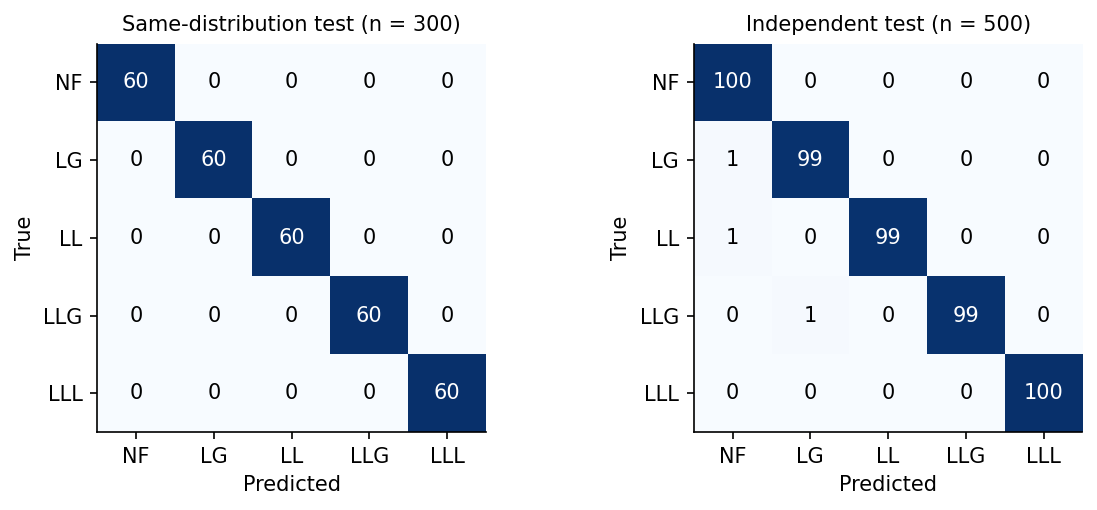
\includegraphics[width=\textwidth]{fig_confusion.png}
\caption{Confusion matrices for the same-distribution test (left) and the independent test (right).}\label{fig:conf}
\end{figure}

When trained only on $R_f \le 10\ \Omega$ and tested above it, accuracy fell to 95.5\% (n = 290), with line-to-ground recall of 77\%: tree models do not extrapolate. Holding out a 3--10\,$\Omega$ band (inside the training range) caused no loss (100.0\%).

\subsection{Fault location}
On the same-distribution test the mean location error was 0.89 $\pm$ 0.11\,km over five random splits (single split 1.10\,km; median 0.66\,km; 85\% within 2\,km). On the independent test it was 1.82\,km (95\% bootstrap interval 1.52--2.13\,km), which is 4.6\% of the line length. The median error is 0.71\,km but the 90th percentile is 4.3\,km, so the mean hides a tail of poorly located faults (77\% are within 2\,km).

The tail comes mainly from fault resistance above the training range. For $R_f \le 50\ \Omega$ the independent-test error is 1.10\,km (n = 365), close to the 0.9--1.1\,km seen on the same-distribution test, whereas for 50--100\,$\Omega$ it is 9.3\,km (n = 35), and these faults contribute 45\% of the total error (Figures~\ref{fig:loc} and~\ref{fig:bins}). Faults outside the 2--38\,km training range have a mean error of 2.95\,km (n = 21) against 1.76\,km elsewhere. When trained on $R_f \le 10\ \Omega$ and tested above, the error was 11.4\,km; for the held-out 3--10\,$\Omega$ band it was 2.43\,km.

\begin{figure}[H]\centering
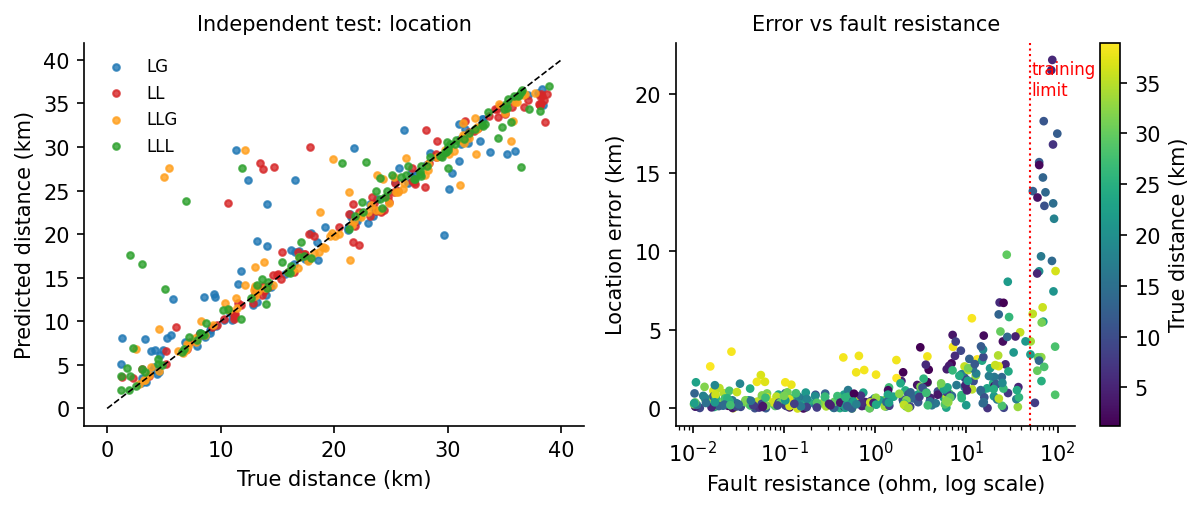
\includegraphics[width=\textwidth]{fig_location.png}
\caption{Independent test. Left: predicted versus true distance. Right: error versus fault resistance; the dotted line marks the training limit.}\label{fig:loc}
\end{figure}

\begin{figure}[H]\centering
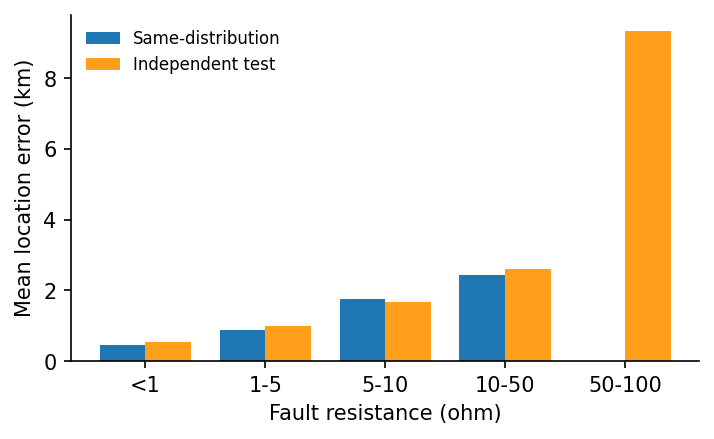
\includegraphics[width=0.65\textwidth]{fig_rf_bins.png}
\caption{Mean location error by fault-resistance band.}\label{fig:bins}
\end{figure}

\subsection{Ablation and classical baseline}
Table~\ref{tab:abl} shows that removing the resistance and reactance features raises the location error from 0.89 to 1.57\,km and, for 10--50\,$\Omega$ faults, from 2.1 to 4.4\,km, supporting the argument in Section~\ref{sec:locbg}. Using the resistance and reactance features alone gives a similar error (0.97\,km); the difference from the full set is within the split-to-split variation. The classical baseline estimates distance as loop reactance divided by $0.5\ \Omega$/km, using the \emph{true} faulted phases. It has a mean error of 1.88\,km (median 1.21\,km) on the training data and 3.09\,km (median 1.51\,km) on the independent set, so the model reduces the mean error by roughly 40--50\%. The baseline has no DC-offset filtering and is not a tuned protection algorithm.

\begin{table}[H]\centering\small
\caption{Location error by feature set (mean over five splits, same-distribution test).}\label{tab:abl}
\begin{tabular}{lcc}\toprule
Feature set & Mean error (km) & Error, 10--50\,$\Omega$ (km)\\\midrule
All features & 0.89 $\pm$ 0.11 & 2.1\\
Without resistance/reactance & 1.57 $\pm$ 0.16 & 4.4\\
Resistance/reactance only (plus $V_1$, $I_1$) & 0.97 $\pm$ 0.09 & 1.6\\\bottomrule
\end{tabular}
\end{table}

\begin{figure}[H]\centering
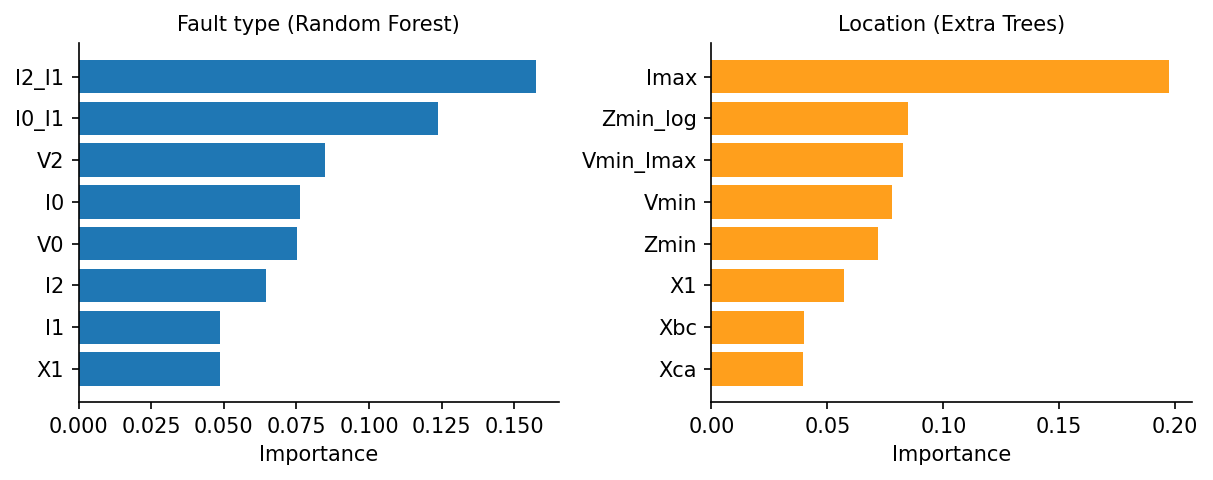
\includegraphics[width=\textwidth]{fig_importance.png}
\caption{Most important features for the type classifier and the locator.}\label{fig:imp}
\end{figure}

\section{Discussion and limitations}
Fault type is easy to recover in this simulator, so the 99.4\% figure should be read as evidence that the pipeline works, not that classification is solved on real systems. Location is the more informative result: about 0.7\,km typical error and 1.8\,km mean on conditions not seen in training, with a clear failure mode at high fault resistance.

The main limitations are as follows.
\begin{itemize}
\item \textbf{Single simulator.} All data come from one Simulink model; the independent test varies operating conditions, not model structure. There are no field data.
\item \textbf{Model simplifications.} The line is lumped RL with zero-sequence impedance equal to positive-sequence (real lines are about 2--3.5 times higher) and no shunt capacitance, which affects ground-fault signatures and the validity of the location features.
\item \textbf{Measurements.} Errors are fixed gains plus Gaussian noise; there is no CT saturation or harmonic content. Phasors are taken from a one-cycle window that includes the decaying DC offset.
\item \textbf{No disturbances.} Load switching, capacitor switching and transformer inrush were not simulated, so the false-alarm result applies only to steady state.
\item \textbf{Class balance.} Classes are balanced; on real systems line-to-ground faults dominate.
\item \textbf{Range.} The models do not extrapolate beyond the fault resistances and locations they were trained on.
\end{itemize}

\subsection{Why noise was introduced}\label{sec:v2}
The first dataset gave 100\% accuracy, which prompted a review. Zero- and negative-sequence quantities in no-fault runs were about $10^{-10}$ (numerically zero), windows were aligned to the known fault time, and the test data came from the same generator as the training data. An ad hoc stress test on the version~1 data (not part of the reproducible scripts), which added a small noise floor to the sequence quantities, reduced a clean-trained classifier to 94\% (2\% floor) and 84\% (5\% floor), indicating that the original result depended on unrealistic symmetry. The update i made adds measurement errors and noise, a trigger that does not know the fault time, resistance and reactance features, and the independent test set.

\section{Conclusion and future work}
A simple pipeline of a current trigger, one-cycle phasor features and tree-based models detects, classifies and locates simulated faults on a 40\,km line with a mean location error of 1.82\,km on an independent test, and its main weakness (fault resistance beyond the training range) is measured rather than hidden. Future work: train over a wider resistance range with a fresh independent test; use a line model with distinct zero-sequence parameters and shunt capacitance; add non-fault disturbances, CT saturation and DC-offset filtering; compare with a tuned classical locator; and validate on field or hardware-in-the-loop data.

\section*{Reproducibility}
Code, data and figures: see the repository README. \texttt{python/evaluate\_and\_figures.py} recomputes every number in this report from the two CSV files (results in \texttt{results/metrics.json}).

\begin{thebibliography}{9}
\bibitem{fortescue1918} C.~L. Fortescue, ``Method of symmetrical co-ordinates applied to the solution of polyphase networks,'' \emph{Trans. AIEE}, vol.~37, no.~2, pp.~1027--1140, 1918.
\bibitem{breiman2001} L.~Breiman, ``Random forests,'' \emph{Machine Learning}, vol.~45, no.~1, pp.~5--32, 2001.
\bibitem{geurts2006} P.~Geurts, D.~Ernst and L.~Wehenkel, ``Extremely randomized trees,'' \emph{Machine Learning}, vol.~63, no.~1, pp.~3--42, 2006.
\bibitem{pedregosa2011} F.~Pedregosa \emph{et al.}, ``Scikit-learn: Machine learning in Python,'' \emph{J. Machine Learning Research}, vol.~12, pp.~2825--2830, 2011.
\bibitem{saha2010} M.~M. Saha, J.~J. Izykowski and E.~Rosolowski, \emph{Fault Location on Power Networks}. London: Springer, 2010.
\end{thebibliography}

\end{document}
